\documentclass{memoria}


\begin{document}

\portada{Diseño de Bases de Datos: Laboratorio 2\\ Análisis de eventos sociales masivos}{Elías González\\José Latapiatt\\ Ian Orellana}{Profesora: Carolina Bonacic \\ Ayudantes: Fabián Arismendi\\ Miguel Cárcamo}{\today}


\indices
\capitulo{Introducción}
En la experiencia anterior, se creo un modelo conceptual con el objetivo de ejemplificar y exponer las distintas entidades y relaciones involucradas en la base de datos de lo que es el sistema que analiza los eventos masivos, vistas de una forma simple e intuitiva.\\
En esta experiencia se busca realizar un modelo que satisfaga los requisitos del sistema, esto es, llevar a cabo distintos procedimientos que den lugar a mayores beneficios o menores costos a la hora de acceder a la base de datos para realizar búsquedas o cualquier otra operación. Junto con esto, se realizan las respectivas consultas que llevara a cabo el sistema para implementar el modelo y se describe el procedimiento de almacenamiento que este lleva a cabo.


\capitulo{Objetivos}

\seccion{Objetivo general}
El objetivo, como segunda etapa parcial del proyecto, consiste en realizar un modelo satisfaciendo los distintos requisitos que se plantearon en la experiencia anterior, describiendo las actividades necesarias para su funcionamiento y posterior conexión con los datos a recoger de twitter.

\seccion{Objetivos específicos}
\begin{itemize}
\item Diseñar un modelo físico de bases de datos, a partir del modelo anterior.
\item Normalizar el modelo creado.
\item Describir el funcionamiento de la API de twitter.
\item Describir las consultas SQL realizadas.
\item Describir el procedimiento de almacenado utilizado.
\end{itemize}


\capitulo{Alcances}
\seccion{Herramientas utilizadas}
\begin{itemize}
\item PowerDesigner (Modeling and Metadata Managment), utilizado para diseñar los distintos modelos.
\end{itemize}

\seccion{Conocimiento necesario}
\begin{itemize}
\item Se utilizan convenciones de modelos de entidad relación para bases de datos relacionales, tanto modelo conceptual como físico.
\item Se utilizan normas convencionales de normalización de tablas de bases de datos.
\item Se utilizan consultas a la base de datos en SQL.
\end{itemize}


\capitulo{Modelos de bases de datos}
\seccion{Modelo conceptual}
El siguiente modelo presenta las entidades y relaciones existentes en la base de datos, a continuación se exhibirá en detalle los atributos correspondiente a cada tabla junto con la descripción de su utilidad para el sistema.\\
\\
\begin{figure}[!ht]
\begin{center}
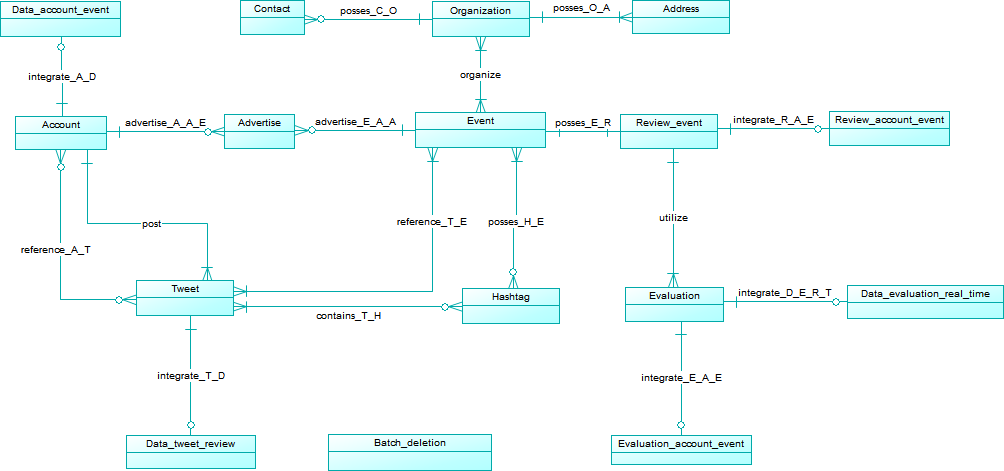
\includegraphics[width=1\textwidth]{img/conceptual.png}
\caption{Modelo Conceptual de bases de datos.}
\end{center}
\end{figure}
\newpage


\begin{figure}[!ht]
\begin{center}
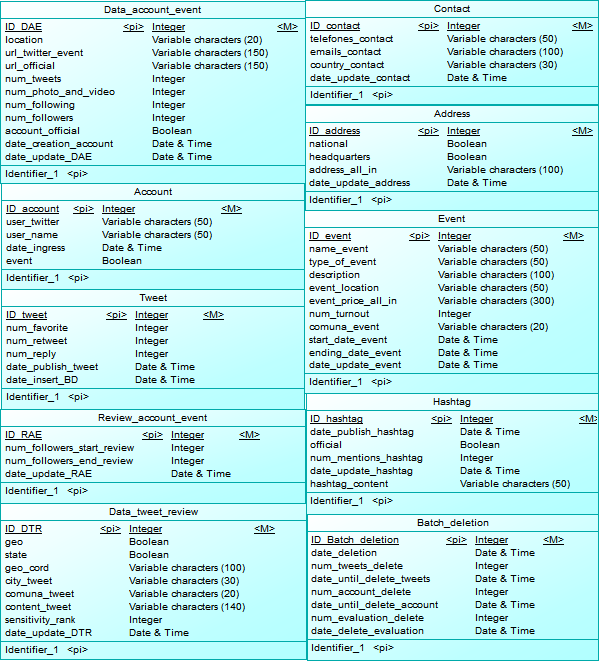
\includegraphics[width=0.9\textwidth]{img/tablaconceptual2.png}
\caption{Entidades y atributos del modelo conceptual. Sección 1}
\end{center}
\end{figure}

\textit{Data\_account\_event}, es una entidad dirigida a soportar datos correspondientes a las cuentas asociadas a los eventos, entre ellos localización, número de tweets, número de seguidores, fechas en que comenzó a publicar y distingue un atributo exclusivo para la página oficial del evento, diferenciándola del que posee el evento en twitter.\\
\textit{Account} contiene los datos específicos de un elemento de estudio, como lo son su twitter y su nombre, además posee un dato tipo \textit{boolean} para identificar si corresponde a una cuenta oficial de un evento.\\
\textit{Tweet} se encarga de contar las veces que un tweet fue retweeteado, compartido o añadido a favoritos, acompañado de su fecha de publicación y .a fecha en que fue añadida a la base de datos. Posee dos tipos de relación con \textit{Account}, puesto que una cuenta puede publicar varios tweets (relación uno a muchos), pero por otro lado, una cuenta puede ser referenciada por varios tweets y a la vez referenciar a muchos otros.\\
\textit{Event} captura datos y características del evento, en su mayor parte son los que no se obtienen de twitter, tales como comuna, tipo de evento o descripción. Además añade fechas de inicio y término si es un evento que se lleva a cabo por más de un día.\\
\textit{Hashtag} almacena información importante de los hashtag, como su contenido, fecha, hora y número de veces que fue mencionado.\\
\textit{Adress} y \textit{Contact}, como su nombre lo indica, guardan información acerca de la dirección física de la organizadora del evento y el contacto por cualquier medio con esta.\\
\textit{Batch\_deletion} la cantidad de tweets que son borrados y la fechas útiles para evaluar cuando un tweet debe ser eliminado de la base de datos.
\newpage

\begin{figure}[!ht]
\begin{center}
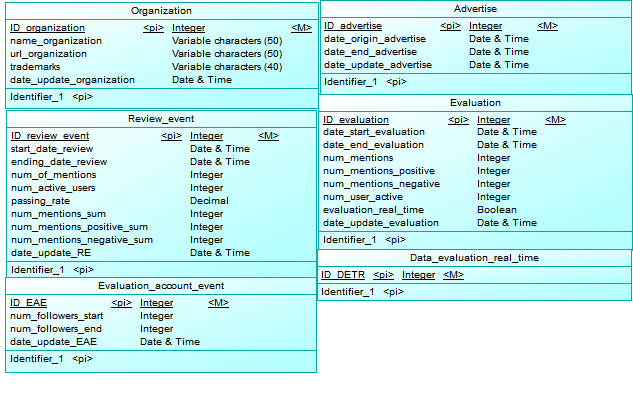
\includegraphics[width=0.9\textwidth]{img/tablaconceptual3.png}
\caption{Entidades y atributos del modelo conceptual. Sección 2}
\end{center}
\end{figure}

\textit{Organización} contiene los datos principales de la organización que dirige el evento, nombre, dirección de su página web y marcas asociadas.\\
\textit{Advertise}, es una tabla que conecta \textit{Account} y \textit{Event}, y almacena las fechas de comienzo y fin de publicidad de un evento por parte de una cuenta.\\
\textit{Evaluation} contiene información sobre el análisis realizado del evento en un plazo determinado, además, algunas evaluaciones servirán para persistir información en tiempo real en caso de falla de sistema, contiene los datos que se usarán para crear las estadísticas de cierto evento de acuerdo a sus menciones positivas o negativas.\\
\textit{Review\_event} posee la información final del análisis realizado para determinado evento, para esto maneja atributos como la cantidad total de las menciones positivas y negativas.\\
\textit{Evaluation\_acount\_event} mantiene el número de seguidores a un evento en un tiempo determinado.\\
\textit{Data\_evaluation\_real\_time}  mantiene información sobre eventuales evaluaciones en tiempo real.

\newpage
\seccion{Modelo físico}
Con el objetivo de producir una descripción base de la implementación de la base de datos, se muestra el modelo físico de bases de datos, el cuál expone además las relaciones de mayor importancia o relaciones base, donde es necesario almacenar ciertos datos puesto que el tipo de relación es de muchos a muchos.\\
\\
\begin{figure}[!ht]
\begin{center}
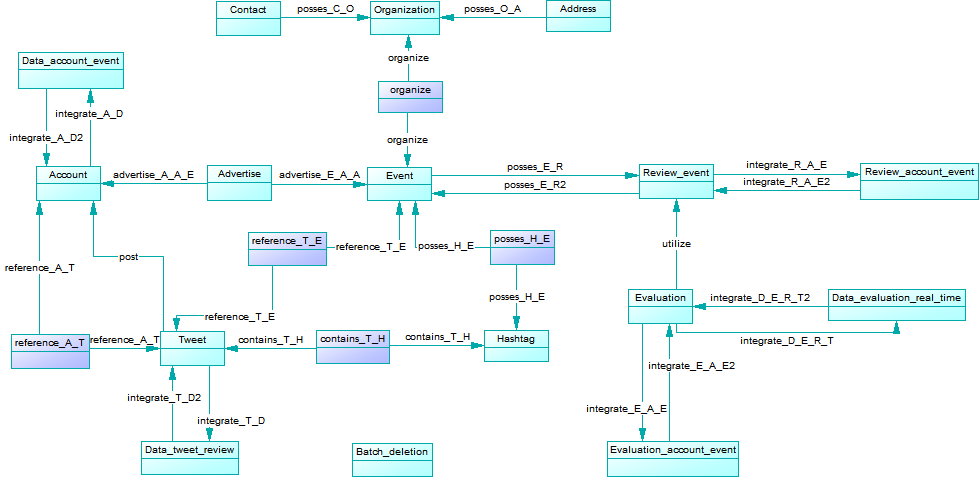
\includegraphics[width=1\textwidth]{img/fisico.png}
\caption{Modelo Físico de bases de datos.}
\end{center}
\end{figure}
\newpage

\begin{figure}[!ht]
\begin{center}
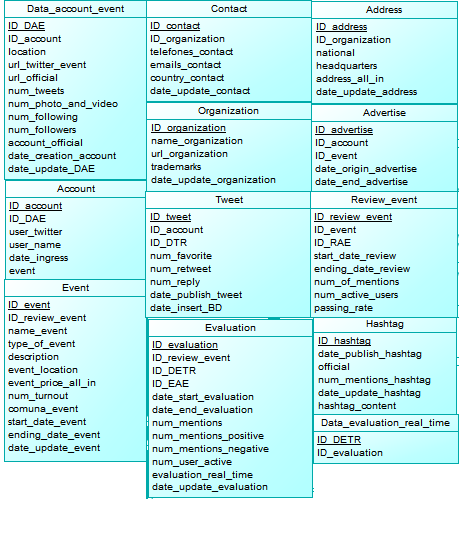
\includegraphics[width=0.9\textwidth]{img/tablafisica2.png}
\caption{Entidades y atributos del modelo físico. Sección 1}
\end{center}
\end{figure}
\newpage
\begin{figure}[!ht]
\begin{center}
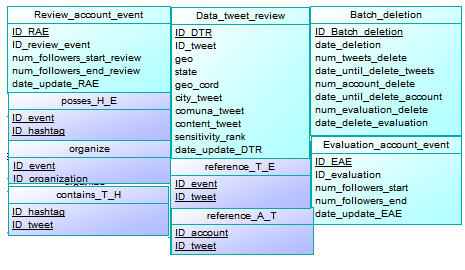
\includegraphics[width=0.9\textwidth]{img/tablafisica3.png}
\caption{Entidades y atributos del modelo físico. Sección 2}
\end{center}
\end{figure}

\textit{reference\_A\_T} es una relación que contiene los identificadores de una cuenta y un tweet que realiza. Esta relación hace referencia a que una cuenta puede referenciar a distintos tweets, y a la vez ser referenciada por varios tweets.\\
\textit{reference\_T\_E} indica que un tweet puede referenciar a varios eventos y un evento puede referenciar a varios tweets. Almacena tanto la identificación del evento como la del tweet.\\
\textit{posses\_H\_E}, indica que un evento puede poseer varios hashtag que lo referencien, y a la vez \\
\textit{contains\_T\_H} hace referencia a la que en un tweet se pueden incluir varios hashtag, y a la vez, un hashtag puede ser referenciado en muchos tweets. Guarda la identificación del tweet y el hashtag utilizado.\\
\textit{organize} ya que una organización puede organizar varios eventos, y a la vez un evento puede estar a cargo de varias organizaciones, esta relación se encarga de guardar las identificaciones tanto de la organización como del evento.
\newpage
\seccion{Descripción de la normalización}
A continuación se mostrarán cada una de las tablas del modelo de bases de datos previamente expuesto seguido de un análisis sobre sus atributos. El proceso de normalización consiste en organizar los atributos y entidades de una forma eficiente en la base de datos, permitiendo mejorar su acceso y evitando errores al agregar o eliminar elementos. El formato mediante el cual se muestran es \textit{Entidad(atributo\_1, atributo\_2....,atributo\_n)}

\begin{itemize}
\item[1.-]\textbf{ Data\_account\_event(ID\_DAE, ID\_account, location, url\_twitter\_event,	 url\_official, num\_tweets,  num\_photo\_and\_video, num\_following, num\_followers,  account\_official, date\_creation\_account, date\_update\_DAE)} \\
Se encuentra en 1FN (Primera forma normal) ya que todos sus datos son atómicos o escalares.\\
Se encuentra en 2FN (Segunda forma normal) ya que está en 1FN, además cada atributo no llave depende de las llaves ID\_DAE, ID\_account (1:1).\\
 Se encuentra en 3FN (Tercera forma normal) ya que cada atributo no llave de la tabla no depende de forma funcional transitiva de la llave primaria.\\ 
Se encuentra en FNBC (Forma normal de Boyce Codd), ya que no hay dependencias por transitividad y en 4FN (Cuarta forma normal) no posee dependencias multi-evaluadas.

\item[2.-]\textbf{Account (ID\_account, ID\_DAE, user\_twitter, user\_name, date\_ingress, event)}
\\
Se encuentra en 1FN ya que todos sus datos son atómicos o escalares.\\
Se encuentra en 2FN ya que está en 1FN, además cada atributo no llave depende de las llaves ID\_account, ID\_DAE, ID\_advertise(1:0 $|$1:0 $|$1). \\
Se encuentra en 3FN ya que cada atributo no llave de la tabla no depende de forma funcional transitiva de la llave primaria. Se encuentra en FNBC,  ya que no hay dependencias por transitividad y en  4FN no posee dependencias multi-evaluadas. 

\item[3.-]\textbf{Tweet(ID\_tweet, ID\_account, ID\_DTR, num\_favorite, num\_retweet, num\_reply, date\_publish\_tweet, date\_insert\_BD)}
\\
Se encuentra en 1FN ya que todos sus datos son atómicos o escalares.\\
Se encuntra en 2FN ya que está en 1FN, además cada atributo no llave depende de las llaves ID\_tweet, ID\_account, ID\_DTR (1:1: 0$|$1). Se encuentra en 3FN ya que cada atributo no llave de la tabla no depende de forma funcional transitiva de la llave primaria. \\
Se encuentra en FNBC, ya que no hay dependencias por transitividad y en 4FN no posee dependencias multi-evaluadas.

\item[4.-]\textbf{Data\_tweet\_review (ID\_DTR, ID\_tweet, geo, state, geo\_cord, city\_tweet, comuna\_tweet, content\_tweet, sensitivity\_rank, date\_update\_DTR)}
\\
Se encuentra en 1FN ya que todos sus datos son atómicos o escalares.
Se encuentra en 2FN ya que está en 1FN, además cada atributo no llave depende de las llaves ID\_DTR, ID\_tweet (1:1). Se encuentra en 3FN ya que cada atributo no llave de la tabla no depende de forma funcional transitiva de la llave primaria. Se encuentra en FNBC,  ya que no hay dependencias por transitividad y en  4FN no posee dependencias multi-evaluadas.

\item[5.-]\textbf{Advertise (ID\_advertise, ID\_account, ID\_event, date\_origin\_advertise, date\_end\_advertise, date\_update\_advertise)}
\\
Se encuentra en 1FN ya que todos sus datos son atómicos o escalares.\\
Se encuentra en 2FN ya que esta en 1FN, además cada atributo no llave depende de las llaves ID\_advertise, ID\_account, ID\_event  (1:1:1).\\
 Se encuentra en 3FN ya que cada atributo no llave de la tabla no depende de forma funcional transitiva de la llave primaria. Se encuentra en FNBC,  ya que no hay dependencias por transitividad y en  4FN no posee dependencias multi-evaluadas.
 
\item[6.-]\textbf{Event (ID\_event, ID\_review\_event, name\_event, type\_of\_event, description, event\_location, event\_price\_all\_in, num\_turnout, comuna\_event, start\_date\_event, ending\_date\_event, date\_update\_event)}
\\
Se encuentra en 1FN ya que todos sus datos son atómicos o escalares.\\
Se encuentra en 2FN ya que esta en 1FN, además cada atributo no llave depende de las llaves ID\_event, ID\_review\_event, ID\_organization, ID\_advertise (1:1:1 : 0$|$1). Se encuentra en 3FN ya que cada atributo no llave de la tabla no depende de forma funcional transitiva de la llave primaria. Se encuentra en FNBC,  ya que no hay dependencias por transitividad y en  4FN no posee dependencias multi-evaluadas.

\item[7.-]\textbf{Organization (ID\_organization, name\_organization,  url\_organization, trademarks,  date\_update\_organization)}
\\
Se encuentra en 1FN ya que todos sus datos son atomicos o escalares.
\\Se encuentra en 2FN ya que esta en 1FN, además cada atributo no llave depende de las llaves ID\_organization. \\
Se encuentra en 3FN ya que esta en 2FN  y cada atributo no llave de la tabla no depende de forma funcional transitiva de la llave primaria. 
\\Se encuentra en FNBC,  ya que no hay dependencias por transitividad y en  4FN no posee dependencias multi-evaluadas.

\item[8.-]\textbf{Address(ID\_address, ID\_organization, national, headquarters, address\_all\_in, date\_update\_address)}
\\
Se encuentra en 1FN ya que todos sus datos son atómicos o escalares.\\
Se encuentra en 2FN ya que esta en 1FN, además cada atributo no llave depende de las llaves ID\_address, ID\_organization (1:*). Se encuentra en 3FN ya que cada atributo no llave de la tabla no depende de forma funcional transitiva de la llave primaria. 
\\Se encuentra en FNBC,  ya que no hay dependencias por transitividad y en  4FN no posee dependencias multi-evaluadas.

\item[9.-]\textbf{Review\_event(ID\_review\_event, ID\_event, ID\_RAE, start\_date\_review, ending\_date\_review, num\_of\_mentions, num\_active\_users, passing\_rate, num\_mentions\_positive\_sum, num\_mentions\_negative\_sum, date\_upgrade\_RE)}
\\
Se encuentra en 1FN ya que todos sus datos son atómicos o escalares.\\
Se encuentra en 2FN ya que esta en 1FN, además cada atributo no llave depende de las llaves ID\_review\_event, ID\_event, ID\_RAE (1:1: 0$|$1).\\
Se encuentra en 3FN ya que cada atributo no llave de la tabla no depende de forma funcional transitiva de la llave primaria. \\
Se encuentra en FNBC,  ya que no hay dependencias por transitividad y en 4FN no posee dependencias multi-evaluadas.

\item[10.-]\textbf{Review\_account\_event(ID\_RAE, ID\_review\_event, num\_followers\_start\_review, num\_followers\_end\_review, date\_update\_review)}
\\
Se encuentra en 1FN ya que todos sus datos son atómicos o escalares.\\
Se encuentra en 2FN ya que esta en 1FN, además cada atributo no llave depende de las llaves ID\_RAE, ID\_review\_event  (1:1) .\\
Se encuentra en 3FN ya que cada atributo no llave de la tabla no depende de forma funcional transitiva de la llave primaria. Se encuentra en FNBC,  ya que no hay dependencias por transitividad y en  4FN no posee dependencias multi-evaluadas.

\item[11.-]\textbf{Evaluation (ID\_evaluation,ID\_review\_event, ID\_DETR, ID\_EAE, date\_start\_evaluation, date\_end\_evaluation, num\_mentions, num\_mentions\_positive, num\_mentions\_negative, num\_user\_active, evaluation\_real\_time, date\_update\_evaluation)}
\\
Se encuentra en 1FN ya que todos sus datos son atómicos o escalares.\\
Se encuentra en 2FN ya que esta en 1FN, además cada atributo no llave depende de las llaves ID\_evaluation,ID\_review\_event, ID\_DETR, ID\_EAE (1:1: 0$|$1 : 0$|$1).\\
Se encuentra en 3FN ya que cada atributo no llave de la tabla no depende de forma fucional transitiva de la llave primaria.\\ 
Se encuentra en 4FN no posee dependencias multievaluadas.

\item[12.-]\textbf{Data\_evaluation\_real\_time (ID\_DETR, ID\_evaluation)}\\
Se encuentra en 1FN ya que todos sus datos son atómicos o escalares.\\
Se encuentra en 2FN ya que esta en 1FN, además cada atributo no llave depende de las llaves ID\_DETR, ID\_evaluation (1:1).\\
Se encuentra en 3FN ya que cada atributo no llave de la tabla no depende de forma funcional transitiva de la llave primaria. \\
Se encuentra en FNBC,  ya que no hay dependencias por transitividad y en 4FN no posee dependencias multi-evaluadas.

\item[13.-]\textbf{Evaluation\_account\_event(ID\_EAE, ID\_evaluation, num\_followers\_start, num\_followers\_end, date\_update\_EAE)}
\\
Se encuentra en 1FN ya que todos sus datos son atómicos o escalares.\\
Se encuentra en 2FN ya que esta en 1FN, además cada atributo no llave depende de las llaves ID\_EAE, ID\_evaluation (1:1).\\
Se encuentra en 3FN ya que cada atributo no llave de la tabla no depende de forma funcional transitiva de la llave primaria. Se encuentra en FNBC,  ya que no hay dependencias por transitividad y en  4FN no posee dependencias multi-evaluadas.

\item[14.-]\textbf{Hashtag(ID\_hashtag, date\_publish\_hashtag, official, num\_mentions\_hashtag, date\_update\_hashtag, hashtag\_content)}
\\
Se encuentra en 1FN ya que todos sus datos son atómicos o escalares.\\
Se encuentra en 2FN ya que esta en 1FN, además cada atributo no llave depende de las llaves ID\_hashtag. \\
Se encuentra en 3FN ya que esta en 2FN y cada atributo no llave de la tabla no depende de forma funcional transitiva de la llave primaria. \\
Se encuentra en FNBC,  ya que no hay dependencias por transitividad y en  4FN no posee dependencias multi-evaluadas.

\item[15.-]\textbf{ Batch\_deletion (ID\_Batch\_deletion, date\_deletion, num\_tweets\_delete, date\_until\_delete\_tweets, num\_account\_delete, date\_until\_delete\_account, num\_evaluation\_delete, date\_delete\_evaluation)}
\\
Se encuentra en 1FN ya que todos sus datos son atómicos o escalares.\\
Se encuentra en 2FN ya que esta en 1FN, ademas cada atributo no llave depende de las llaves ID\_Batch\_deletion.\\ Se encuentra en 3FN ya que esta en 2FN y cada atributo no llave de la tabla no depende de forma funcional transitiva de la llave primaria.\\
Se encuentra en FNBC, ya que no hay dependencias por transitividad y en 4FN no posee dependencias multi-evaluadas.

\item[16.-]\textbf{Reference\_A\_T (ID\_account, ID\_tweet)}
\\
Se encuentra en 1FN ya que todos sus datos son atómicos o escalares.\\
Se encuentra en 2FN ya que esta en 1FN, además cada atributo no llave depende de las ID\_account, ID\_tweet.\\
Se encuentra en 3FN ya que cada atributo no llave de la tabla no depende de forma funcional transitiva de la llave primaria. \\
Se encuentra en FNBC,  ya que no hay dependencias por transitividad y en  4FN no posee dependencias multi-evaluadas.

\item[17.-]\textbf{Reference\_T\_E (ID\_event, ID\_tweet)}
\\
Se encuentra en 1FN ya que todos sus datos son atómicos o escalares.\\
Se encuentra en 2FN ya que esta en 1FN, además cada atributo no llave depende de las ID\_event, ID\_tweet. \\
Se encuentra en 3FN ya que cada atributo no llave de la tabla no depende de forma funcional transitiva de la llave primaria. \\
Se encuentra en FNBC,  ya que no hay dependencias por transitividad y en  4FN no posee dependencias multi-evaluadas.

\item[18.-]\textbf{Contains\_T\_H (ID\_hashtag, ID\_tweet)}
\\
Se encuentra en 1FN ya que todos sus datos son atómicos o escalares.\\
Se encuentra en 2FN ya que esta en 1FN, además cada atributo no llave depende de las ID\_hashtag, ID\_tweet.\\
Se encuentra en 3FN ya que cada atributo no llave de la tabla no depende de forma funcional transitiva de la llave primaria. \\
Se encuentra en FNBC, ya que no hay dependencias por transitividad y en  4FN no posee dependencias multi-evaluadas.

\item[19.-]\textbf{Organize (ID\_event, ID\_organization)}
\\
Se encuentra en 1FN ya que todos sus datos son atómicos o escalares.\\
Se encuentra en 2FN ya que esta en 1FN, además cada atributo no llave depende de las ID\_event, ID\_organization. \\Se encuentra en 3FN ya que cada atributo no llave de la tabla no depende de forma funcional transitiva de la llave primaria.\\ Se encuentra en FNBC,  ya que no hay dependencias por transitividad y en  4FN no posee dependencias multi-evaluadas.\\

\item[20.-]\textbf{Posses\_H\_E (ID\_event, ID\_hashtag)}
\\
Se encuentra en 1FN ya que todos sus datos son atómicos o escalares.\\
Se encuentra en 2FN ya que esta en 1FN, además cada atributo no llave depende de las ID\_event, ID\_hashtag.\\ Se encuentra en 3FN ya que cada atributo no llave de la tabla no depende de forma funcional transitiva de la llave primaria. \\Se encuentra en FNBC,  ya que no hay dependencias por transitividad y en  4FN no posee dependencias multi-evaluadas.

\item[21.-]\textbf{Contact (ID\_contact, ID\_organization, Phones\_contact, emails\_contact, country\_contact)}
\\
Se encuentra en 1FN ya que todos sus datos son atómicos o escalares.
Se encuentra en 2FN ya que esta en 1FN, además cada atributo no llave depende de las ID\_contact, ID\_organization.\\ Se encuentra en 3FN ya que cada atributo no llave de la tabla no depende de forma funcional transitiva de la llave primaria.\\ Se encuentra en FNBC,  ya que no hay dependencias por transitividad y en  4FN no posee dependencias multi-evaluadas.
\end{itemize}

\capitulo{Descripción y funcionamiento de la API}
Twitter cuenta con 3 tipos de APIs, Search API, REST API y Streaming API, para nuestro proyecto se utilizarán las dos últimas, de estas dos, cada una tiene su utilidad particular que se procederá a explicar a continuación.\\



La REST API es de las dos que será utilizada y la que posee más funcionalidades. Por otro lado, su mayor restricción, un uso de máximo 350 usos por hora de forma autentificada, lo que imposibilita usarla para todos los requerimientos. En particular esta API puede ser utilizada para subir tweets, agregar localización, seguir gente, crear listas, a grandes razgos lo que puede hacer un usuario de twitter desde el sitio web, incluyendo la búsqueda de contenido. Cabe destacar el hecho de que esta API al buscar, permite conseguir Tweets de una antigüedad superior a la streaming API, con un máximo actual de 3200 Tweets. Su utilidad para el proyecto involucra la obtención de los datos de las cuentas de los eventos.\\

La Streaming API en cambio, permite mantenerse conectados a Twitter y recibir los Tweets con keywords, configuraciones de locación e idioma que son requeridas, recibiendo los datos casi en tiempo real en comparación a lo que se esta subiendo a Twitter. Es decir, se recibe información del flujo de la misma que es al final el servicio de Twitter. En este caso la limitante esta que no se puede conseguir los tweets más antiguos con respecto a un tema, para ello se ocupará la Rest API. Esta API es particularmente efectiva en trabajos de minería de datos, de análisis de grandes cantidades de tweets a través del tiempo, que es lo que se espera lograr con el proyecto.
La streaming API tiene a su vez tres grandes formas de usarse, statuses\/firehose que es un gran flujo de toda la información recibida por twiter sin mayores filtros, statuses\/sample que entrega una muestra aleatoria de lo que se busca y un filtrado (statuses\/filter)  a base de keywords, a estas también se puede ocupar statuses/links para obtener solo tweets que incluyan links o statuses\/retweet para obtener solo tweets que sean retweets, lo que ayudara a separar estos tipos de tweets para generar las estadísticas mencionadas en los requerimientos del sistema.\\
Para conectarse con la API de Twiter se utiliza RUBY on Rails, en particular las gema Twiter.


\capitulo{Descripción de la aplicación}
Las funciones que el sistema debe implementar incluyen la exposición en cada sección correspondiente a un evento, de sus atributos convencionales, ubicación, precio de entradas, empresa organizadora, fecha, hora y tipo de evento (musical (género), deportivo, artístico); Además debe obtener el número de seguidores de cada evento, número al cuál el usuario puede acceder.\\
El sistema debe clasificar los tweets según su intención positiva o negativa, y exponer dicha clasificación mediante una estadística simple de porcentajes apoyada por un gráfico de torta.\\
El sistema debe monitorear los tweets referidos a un evento, controlando la fecha y hora de su emisión para luego, con la ayuda de un gráfico de líneas, tener la posibilidad de acceder a la forma en que se altera el volumen de tweets emitidos a lo largo del tiempo, o por un periodo de tiempo a seleccionado por el usuario.\\
El sistema debe mostrar un ránking con los 10 eventos que posean más tweets, así como los hashtags más utilizados.\\
El sistema debe proveer una vista que permita al usuario seleccionar el tipo de evento que quiere observar.\\
El sistema debe incluir una vista donde se muestren los tweets emitidos de cierto evento geo-localizados en un mapa.\\
El objetivo del observatorio es principalmente el de poder realizar comparaciones entre los distintos eventos para crear un fácil análisis de los eventos más populares y sus posibles causas. El incluir la medición del volumen de tweets a través del tiempo, contribuye al estudio del impacto que causan estos eventos durante ciertos periodos, y pueden denotar eventos importantes que hicieron que en cierto momento se hablara con mayor frecuencia sobre cierto evento. El objetivo de la geo-localización es proporcionar información útil para usuarios interesados en realizar estudios sociales que involucren tendencias de sectores de la región a asistir a cierto tipo de eventos o para la empresa organizadora, ya que entrega un indicio de los sectores que comentan más el evento que organizan, dato que puede ser de utilidad para organizar publicidad.

\capitulo{Descripción de consultas SQL}
En esta sección se exhibirán consultas SQL realizadas en la aplicación utilizando Ruby on Rails, junto a una descripción de su utilidad para completar los objetivos de la aplicación.
\begin{itemize}
\item Obtener eventos más populares:
\begin{verbatim}
a = ReviewEvent.order('num\_of\_mentions').pluck(:id)
b = Event.where('id = ?', a).pluck(:name\_event)
b.limit(10)
\end{verbatim}
Obtiene el número de menciones de la tabla ReviewEvent, utilizándolo como criterio de orden descendente, exhibiendo solo los 10 primeros tweets con más menciones. En otras palabras, obtiene los 10 eventos con más menciones, que serán incluidos como $"$los más populares$"$ dentro de la aplicación.

\item Seleccionar el tipo de evento
\begin{verbatim}
c = Event.where('type\_of\_event = ?', '<TIPO>')
\end{verbatim}
Obtiene la tabla con los eventos que pertenecen al tipo de evento seleccionado por el usuario. 

\item Tweets por periodo de tiempo
\begin{verbatim}
d = Tweet.where('date\_publish\_tweet > ? AND 
date\_publish\_tweet < ?', datetime1, datetime2)
\end{verbatim}
Obtiene de la tabla tweets, aquellos datos que cumplan con las restricciones de tiempo ingresadas. Esta consulta entrega los datos útiles para usuarios que se interesan en la cantidad de tweets emitidos durante cierto periodo, y en el caso de requerir la variación de volumen a lo largo del tiempo, se obtienen el nombre del evento y la fecha y hora en que el tweet fue emitido.

\item Obtener cantidad de tweets positivos o negativos del evento
\begin{verbatim}
e = Event.where('name\_event = ?', '<NombreEvento>')
.pluck(:id)
\end{verbatim}
Primero se obtiene el id de la tabla Event (que guarda los datos del evento), donde el atributo name\_event (nombre del evento) coincida con el campo NombreEvento.
\begin{verbatim}
f = ReferenceTE.where('event\_id = ?', e).
pluck(:tweet\_id)
\end{verbatim}
El siguiente paso es, obtener el identificador del tweet de cada tweet presente en la tabla ReferenceTE, cuyo identificador del evento coincida con el de la tabla de datos obtenida anteriormente.
\begin{verbatim}
g = DataTweetReview.where('tweet\_id = ? AND 
sensitivity\_rank = ?',f,0).count
\end{verbatim}
Finalmente se cuentan los tweets de la tabla DataTweetReview donde son contados los tweets cuyo sensivity\_rank corresponda con el valor que desea ser estudiado. Este atributo solo posee dos valores posibles, 1 y 0, de esta forma se guardan con valor 1 los comentarios considerados negativos y con un 0 los positivos.
\end{itemize}


\capitulo{Descripción de triggers utilizados}
Los \textit{triggers} utilizados para este sistema pueden dividirse en dos tipos, aquellos que son utilizados cuando la base de datos esta vacía (\textit{INSERT ON}, ubicados en el archivo adjunto [\textit{TriggersAllInInsert.sql}]), y aquellos que se usan una vez que se ha poblado la base de datos (\textit{UPDATE ON}, ubicados en el archivo adjunto [\textit{TriggersAllInUpdate.sql}]).\\ 
Los \textit{triggers} se usan para lanzar ciertas acciones en el momento que se realiza alguna operación en la base de datos, los procedimientos \textit{INSERT ON}, como su nombre lo indica, insertan datos en tablas de la base de datos cuando estas están vacías, y \textit{UPDATE ON}, actualiza estos campos. A continuación se expone una muestra del código perteneciente a los \textit{triggers} utilizados para el sistema.

\begin{figure}[!ht]
\begin{center}
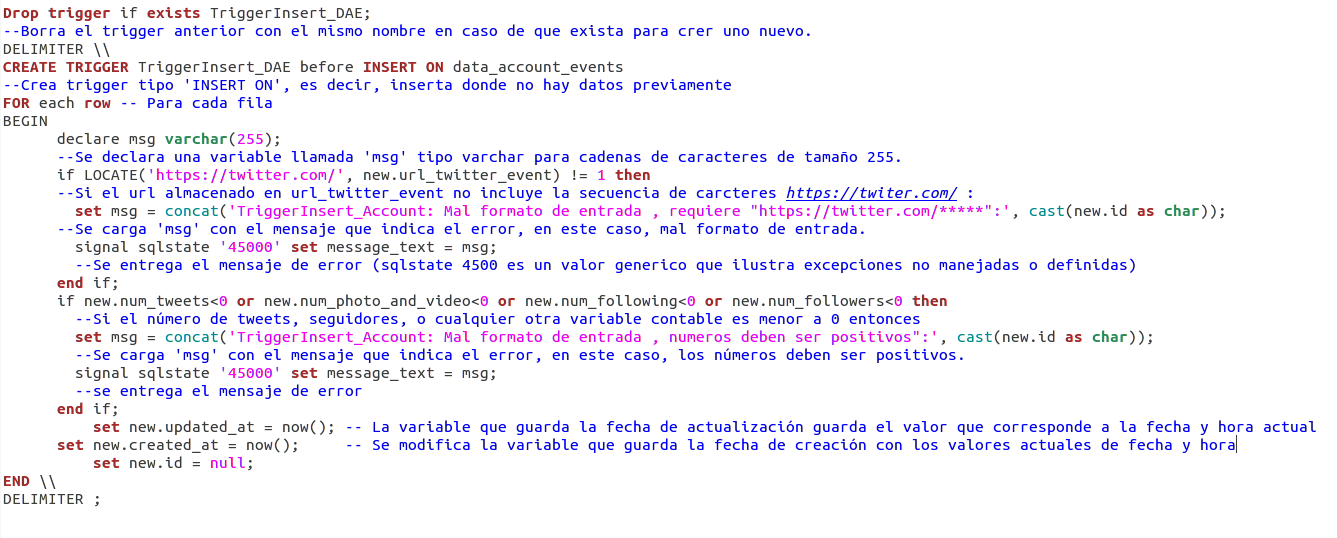
\includegraphics[width=1.2\textwidth]{img/triggerinsert.png}
\caption{Trigger \textit{INSERT ON}}
Extracto del archivo adjunto \textit{TriggersAllInsert}.
\end{center}
\end{figure}
\newpage
\begin{figure}[!ht]
\begin{center}
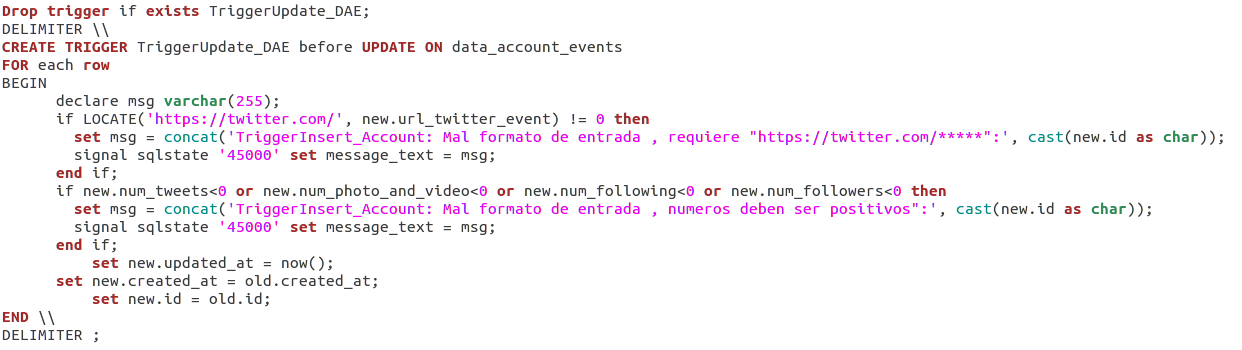
\includegraphics[width=1\textwidth]{img/triggerupdate.png}
\caption{Trigger \textit{UPDATE ON}}
Extracto del archivo adjunto \textit{TriggersAllUpdate}.
\end{center}
\end{figure}
Como se puede observar, la única diferencia de este código con el anterior es que se crea utilizando UPDATE ON en lugar de INSERT ON, es decir, se utiliza para actualizar la tabla pero el procedimiento para agregar un elemento es el mismo. Además, la fecha de actualización en el \textit{trigger} UPDATE ON es modificada, mientras que se mantiene la fecha de creación (\textit{ set new.created\_at = old.created\_at}) y la identidad (\textit{set new.id = old.id}). 
\capitulo{Conclusión}
Se logra crear un modelo adecuado para almacenar los datos requeridos, normalizado y sin pérdida de información.\\
Se identifican las API a utilizar, necesarias para los tipos de datos que se determina obtener, la REST API para obtener datos de eventos y tweets antiguos con respecto a un tema, y streaming API para analizar grandes flujos de datos para generar datos estadísticos propuestos en los objetivos del sistema.\\
Puesto que la mayoría de los objetivos de la aplicación se relacionan con comparaciones entre los eventos, relacionando la magnitud de tweets que reciben, se crear consultas sql que permiten obtener los datos necesarios para cumplir con los requerimientos funcionales que posee el sistema.\\ 

\capitulo{Referencias}
\url  \ Twitter\ Developers (2014). GET statuses/firehose. [ONLINE] Available\ at:\\ https://dev.twitter.com/streaming/reference/get/statuses/firehose. [Last Accessed e.g. 31 August 11].\\
\url  \ ©\ 2014\ Twitter,\ Inc. Twitter API limits. [ONLINE] Available\ at:\\  https://support.twitter.com/articles/160385-twitter-api-limits\# [Last Accessed e.g. 31 August 11].\\
\url   \ Active\ Record\ Query\ Interface\ [ONLINE] Available\ at:\\ http://guides.rubyonrails.org/active\_record\_querying.html [Last Accessed e.g. 31 August 11].\\


\end{document}
